%-------------------------------------------------------------------------------
% Part: FORMATS
%-------------------------------------------------------------------------------
\part{FORMATS}


\chapter{Overview}
\label{cha:formats-overview}

\texttt{FORMATS} contains classes to manage the different formats and
the actual implementation of these formats.

Each format has a format, a writer and a reader object and a unique
name. It also provides a feature which can detect if the format can
read a certain XML document.

There is a special format called ``Error'' which is used whenever an
error occurs.

See figure \ref{fig:formats} for an overview of the cluster.

\begin{figure}[htbp]
  \centering
  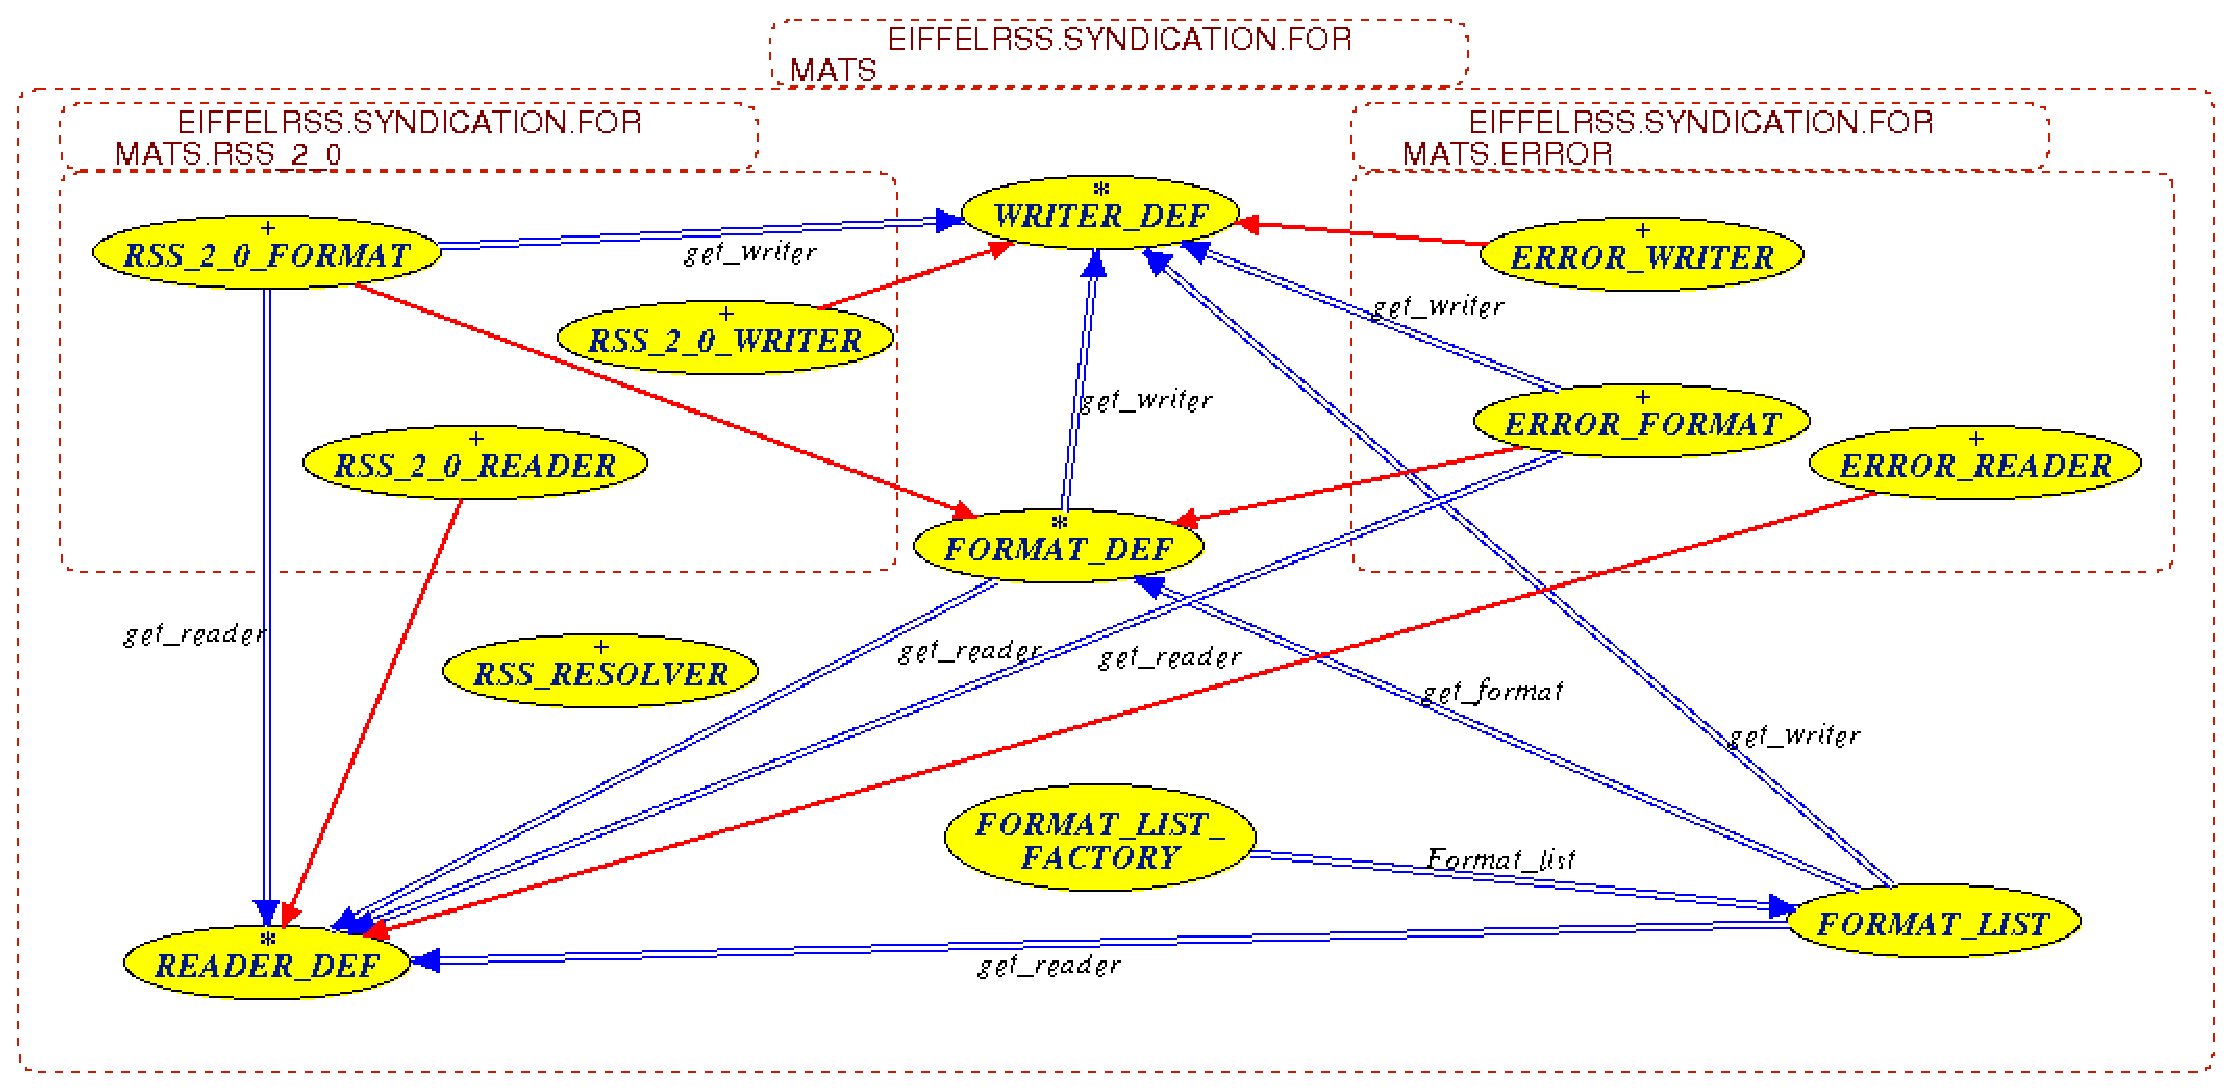
\includegraphics[width=\textwidth]{./figures/EIFFELRSS_SYNDICATION_FORMATS}
  \caption{BON diagram of cluster \texttt{FORMATS}}
  \label{fig:formats}
\end{figure}


\chapter{Management: Class FORMAT\_LIST}
\label{cha:management}


\section{Overview}
\label{sec:management-overview}

\texttt{FORMAT\_LIST} manages the different formats.


\section{Usage}
\label{management-usage}

\texttt{FORMAT\_LIST} uses a singleton pattern, so to actually use the
format list your class has to inherit from
\texttt{FORMAT\_LIST\_FACTORY}.

\texttt{FORMAT\_LIST} inherits from \texttt{LINKED\_LIST}, so all the
features of \texttt{LINKED\_LIST} are availabe as well.


\section{Features}
\label{sec:management-features}


\subsection{Initialization}
\label{sec:management-initialization}

\subsubsection{make\_list}

\begin{lstlisting}[language=Eiffel]
make_list
  -- Create the object and add the default formats
\end{lstlisting}


\subsection{Access}
\label{sec:management-access}

\subsubsection{get\_reader}

\begin{lstlisting}[language=Eiffel]
get_reader (a_name: STRING): READER_DEF
  -- Get the reader object for the name `a_name'
\end{lstlisting}

\subsubsection{get\_writer}

\begin{lstlisting}[language=Eiffel]
get_writer (a_name: STRING): WRITER_DEF
  -- Get the writer object for the name `a_name'
\end{lstlisting}

\subsubsection{get\_format}

\begin{lstlisting}[language=Eiffel]
get_format (a_name: STRING): FORMAT_DEF
  -- Get the format object for the name `a_name'
\end{lstlisting}


\subsection{Detection}
\label{sec:management-detection}

\subsubsection{detect\_format}

\begin{lstlisting}[language=Eiffel]
detect_format (a_document: XM_DOCUMENT): STRING
  -- Get the format name for `a_document'
\end{lstlisting}


\chapter{Format implementations}
\label{cha:formats-implementations}


\section{Addding a new format}
\label{sec:formats-new-format}

Adding a new format to EiffelRSS? is very easy. You have to provide
three objects which inherit from the deferred base classes
\texttt{FORMAT\_DEF}, \texttt{READER\_DEF} and \texttt{WRITER\_DEF}.
If you only want to implement a reader or a writer, you can return
\texttt{ERROR\_WRITER} respectively \texttt{ERROR\_READER} for the
other feature.

To actually add the format to the library, you have to extend
\texttt{FORMAT\_LIST} with an object of the format class.


\section{Base classes}
\label{sec:formats-base-classes}


\subsection{FORMAT\_DEF}
\label{sec:formats-format-def}

\subsubsection{get\_reader}

\begin{lstlisting}[language=Eiffel]
get_reader: READER_DEF
  -- Return a reader object
deferred
\end{lstlisting}

\subsubsection{get\_writer}

\begin{lstlisting}[language=Eiffel]
get_writer: WRITER_DEF
  -- Return a writer object
deferred
\end{lstlisting}

\subsubsection{get\_name}

\begin{lstlisting}[language=Eiffel]
get_name: STRING
  -- Return the format name
deferred
\end{lstlisting}

\subsubsection{is\_of\_format}

\begin{lstlisting}[language=Eiffel]
is_of_format (a_document: XM_DOCUMENT): BOOLEAN
  -- Is this document a feed of our type?
\end{lstlisting}


\subsection{READER\_DEF}
\label{sec:formats-reader-def}

\subsubsection{read}

\begin{lstlisting}[language=Eiffel]
read (a_document: XM_DOCUMENT): FEED
  -- Parse the document and return a feed
deferred
\end{lstlisting}

\subsubsection{get\_name}

\begin{lstlisting}[language=Eiffel]
get_name: STRING
  -- Return a string with the format name
deferred
\end{lstlisting}

\subsubsection{read\_or\_default\_element}

\begin{lstlisting}[language=Eiffel]
read_or_default_element (a_element: XM_ELEMENT; default_value: STRING): STRING
  -- Read the text of `a_element' or use `default_value' if `a_element' is Void or empty
\end{lstlisting}

\subsubsection{read\_or\_default\_attribute}

\begin{lstlisting}[language=Eiffel]
read_or_default_attribute (a_attribute: XM_ATTRIBUTE; default_value: STRING): STRING
  -- Read the value of `a_attribute' or use `default_value' if `a_element' is Void or empty
\end{lstlisting}

\subsubsection{valid\_element\_text}

\begin{lstlisting}[language=Eiffel]
valid_element_text (an_element: XM_ELEMENT; a_name: STRING): BOOLEAN
  -- Has the subelement `a_name' of `an_element' text?
\end{lstlisting}

\subsubsection{read\_date}

\begin{lstlisting}[language=Eiffel]
read_date (a_string: STRING): DATE_TIME
  -- Convert an RFC 822 date string to a DATE_TIME object
\end{lstlisting}


\subsection{WRITER\_DEF}
\label{sec:formats-writer-def}

\subsubsection{get\_name}

\begin{lstlisting}[language=Eiffel]
get_name: STRING
  -- Return a string with the format name
deferred
\end{lstlisting}

\subsubsection{writer}

\begin{lstlisting}[language=Eiffel]
write (a_feed: FEED): XM_DOCUMENT
  -- Export `a_feed' into an xml document
deferred
\end{lstlisting}


\section{Built-in formats}
\label{sec:formats-built-in}


\subsection{RSS 2.0}
\label{sec:formats-rss2}

\texttt{RSS\_2\_0\_FORMAT} is an example implementation of the RSS 2.0
standard. It reads almost all the possible data and has a very basic
writer.


\subsection{Error}
\label{sec:formats-error}

\texttt{ERROR\_FORMAT} is a special format which is used whenever an
error occurs. This removes a lot of sources of errors because the
library can ensure that the reader and writer objects are never
\texttt{Void}.

\texttt{ERROR\_READER} returns a generated feed which has one item
with the error message as description.